\documentclass[11pt]{article}

\usepackage[margin=1in]{geometry}
\usepackage[T1]{fontenc}
\usepackage{lmodern}
\usepackage{graphicx}
\usepackage{booktabs}
\usepackage{array}
\usepackage{caption}
\usepackage{subcaption}
\usepackage{enumitem}
\usepackage{hyperref}
\usepackage{xcolor}
\usepackage{pgfplots}
\usepackage{tikz}
\usepackage{amsmath}
\usepackage{float}
\usepackage{longtable}
\usepackage{tabularx}
\usepackage{ragged2e}

\usetikzlibrary{arrows.meta,positioning,shapes.geometric,fit,calc}
\pgfplotsset{compat=1.18}
\graphicspath{{repo/screenshots/}}
\hypersetup{
    colorlinks=true,
    linkcolor=blue!60!black,
    urlcolor=blue!60!black,
    citecolor=blue!60!black
}

\definecolor{navy}{HTML}{123B5D}
\definecolor{gold}{HTML}{C28C2D}
\definecolor{softblue}{HTML}{EAF2F8}
\definecolor{softgray}{HTML}{F5F6F8}
\definecolor{softgreen}{HTML}{EAF7EE}
\definecolor{softred}{HTML}{FCEEEE}

\newcommand{\callout}[2]{%
\begin{center}
\fcolorbox{navy}{softgray}{%
\parbox{0.94\linewidth}{%
\textbf{#1}\par
\vspace{0.35em}
#2
}}
\end{center}
}

\newcolumntype{Y}{>{\RaggedRight\arraybackslash}X}

\title{From Deepfake Detector to Authenticity Shield\\Single-Document Mini-Capstone}
\author{Abdulrahman Soliman}
\date{}

\begin{document}

\maketitle

\section{Part 1: Executive Summary and Academic Abstract}

\subsection{Executive Summary}
This mini-capstone began as a deepfake image detector and turned into a larger question about \emph{authenticity}. My original goal was straightforward: train, analyze, and deploy a model that could separate \textbf{real} from \textbf{fake} images. I worked with the OpenForensics dataset and the preserved artifacts in this repository, compared CNN candidates, selected the strongest model, and packaged it into a live Streamlit app.

The best preserved model was an \textbf{EfficientNetV2-B0} classifier. It reached \textbf{0.9651 validation accuracy}, \textbf{0.9919 validation precision}, and \textbf{0.9824 validation AUC}. On a harder held-out test set, performance dropped to \textbf{0.8577 accuracy}. That mattered, but the most important moment came later, when I stress-tested the app with a visually plausible but historically impossible image: \textbf{Mahatma Gandhi taking a selfie}. The detector still leaned toward ``real.'' That result changed the project.

It showed me that an image-level detector can learn \emph{visual realism} without learning \emph{historical truth}, \emph{claim consistency}, or \emph{source trust}. In other words, strong deepfake detection is not the same thing as strong authenticity assessment.

\callout{Main Finding}{
My first-iteration system works as an image-level forensic detector, but the Gandhi selfie stress test showed that forensic realism alone is too narrow to judge authenticity.
}

\callout{What Changed My Thinking}{
The project stopped being only ``can I detect deepfakes from pixels?'' and became ``what kinds of evidence are needed to decide whether AI-generated or manipulated media should be trusted?''
}

What comes next is a four-layer image authenticity system with:
\begin{itemize}[leftmargin=1.5em]
    \item forensic evidence,
    \item semantic consistency checks,
    \item context and claim verification,
    \item provenance and metadata signals.
\end{itemize}

\begin{figure}[H]
\centering
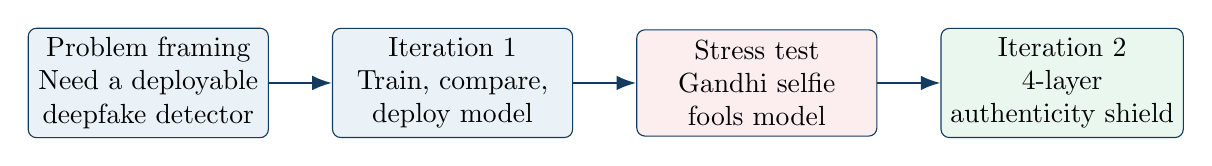
\begin{tikzpicture}[
    node distance=1.9cm and 0.8cm,
    box/.style={draw=navy, rounded corners=3pt, align=center, minimum width=3.05cm, minimum height=1.35cm, fill=softblue},
    arrow/.style={-{Latex[length=2.5mm]}, thick, draw=navy}
]
\node[box] (a) {Problem framing\\Need a deployable\\deepfake detector};
\node[box, right=of a] (b) {Iteration 1\\Train, compare,\\deploy model};
\node[box, right=of b, fill=softred] (c) {Stress test\\Gandhi selfie\\fools model};
\node[box, right=of c, fill=softgreen] (d) {Iteration 2\\4-layer\\authenticity shield};
\draw[arrow] (a) -- (b);
\draw[arrow] (b) -- (c);
\draw[arrow] (c) -- (d);
\end{tikzpicture}
\caption{The capstone arc: I started with a deployable deepfake detector, then used a failure case to motivate a broader authenticity system.}
\label{fig:project-arc}
\end{figure}

\subsection{Academic Abstract}
This mini-capstone documents the first iteration of a deployable deepfake image detector and the conceptual pivot it produced. Using the OpenForensics dataset and preserved repository artifacts, I audited and operationalized a CNN-based image classification pipeline for real-vs-fake detection. The project compared multiple CNN architectures and selected \textbf{EfficientNetV2-B0} as the strongest preserved model. The chosen model used transfer learning from ImageNet, a binary sigmoid output head, image resizing to \textbf{256 $\times$ 256}, in-model normalization, and selected augmentation during training. Preserved evaluation artifacts report \textbf{0.9651 validation accuracy}, \textbf{0.9919 validation precision}, and \textbf{0.9824 validation AUC}; on a harder held-out test set, performance dropped to \textbf{0.8577 accuracy}, highlighting sensitivity to distribution shift and post-processing.

The most important outcome of the project was not only the deployed detector, but the limitation revealed through qualitative stress testing. A historically impossible but visually plausible synthetic image --- Mahatma Gandhi taking a selfie --- was still judged as real by the first-iteration system. This clarified that image-level forensics and authenticity verification are not the same task. I therefore reframe the next iteration as a layered image-authenticity architecture combining low-level forensic modeling, semantic consistency checks, contextual verification, and provenance analysis. The completed work product is a strong first-layer detector and a detailed account of the evidence needed to extend it into a more trustworthy system.

\clearpage
\tableofcontents
\clearpage

\section{Part 2: Capstone Work Product}

\subsection{Problem / Idea}
The first version of the project asked a narrow and defensible question:
\begin{quote}
Can I build and deploy a strong image-level detector that separates real and fake images using preserved deep learning artifacts from this repository?
\end{quote}

That question mattered for two reasons. First, deepfake detection is already a meaningful applied machine learning problem. Second, it gave me a concrete first layer for a broader system I had in mind. I did not want to start from a vague ``AI shield'' concept. I wanted to start from a working model, deploy it, and then find out where it broke.

By the end of the project, the sharper question became:
\begin{quote}
What evidence is actually needed to judge the authenticity of an image, rather than only its visual realism?
\end{quote}

That sharper question came from the work product itself. It was not only an abstract idea added later.

\subsection{Approach / Method}

\subsubsection{Why this dataset was the right first choice}
The project uses \textbf{OpenForensics}, a large-scale benchmark for face forgery detection and segmentation in the wild \cite{le2021openforensics}. It was a good first dataset because:
\begin{itemize}[leftmargin=1.5em]
    \item it already supported supervised real-vs-fake classification,
    \item it was large enough to compare several CNN candidates,
    \item it let me focus on the model and deployment pipeline before solving the harder multi-source data integration problem.
\end{itemize}

In the preserved training notebooks, the working split was:
\begin{itemize}[leftmargin=1.5em]
    \item \textbf{140,002} training images,
    \item \textbf{39,428} validation images,
    \item \textbf{10,905} test images.
\end{itemize}

That made the current iteration a substantial image-classification project, while still being narrower than the full authenticity system I plan to build next.

\begin{figure}[H]
\centering
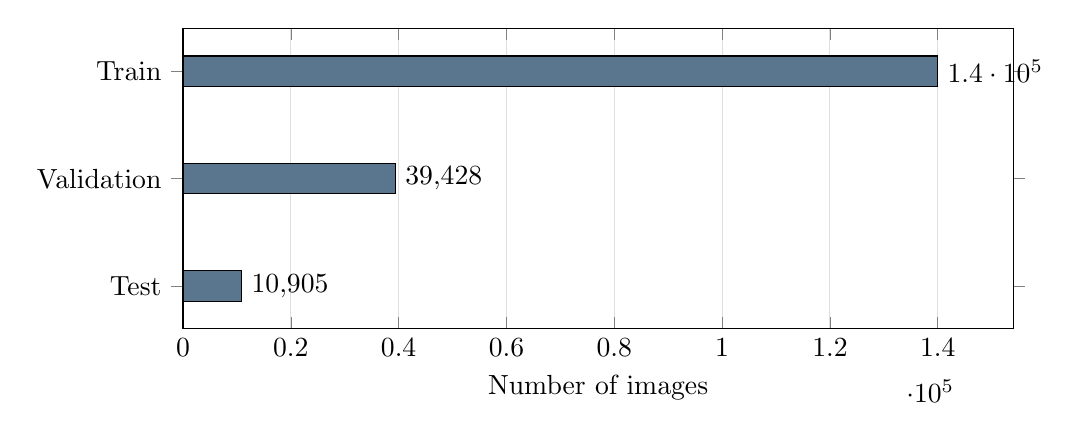
\begin{tikzpicture}
\begin{axis}[
    xbar,
    width=\textwidth,
    height=5.4cm,
    xmin=0,
    xlabel={Number of images},
    symbolic y coords={Test,Validation,Train},
    ytick=data,
    nodes near coords,
    nodes near coords align={horizontal},
    bar width=11pt,
    enlarge y limits=0.2,
    xmajorgrids=true,
    grid style={gray!25}
]
\addplot[fill=navy!70] coordinates {(10905,Test) (39428,Validation) (140002,Train)};
\end{axis}
\end{tikzpicture}
\caption{OpenForensics split used in the preserved training pipeline.}
\label{fig:data-split}
\end{figure}

\subsubsection{Preprocessing pipeline}
The preserved notebooks and saved model files show a stable preprocessing pipeline:
\begin{itemize}[leftmargin=1.5em]
    \item directory-based binary label loading,
    \item image resizing to \textbf{256 $\times$ 256},
    \item batch size of \textbf{64},
    \item in-model rescaling and normalization,
    \item data augmentation for selected models, including \textbf{horizontal flips} and \textbf{rotations}.
\end{itemize}

This matters because a CNN comparison only means something if the inputs are standardized. The project did not depend on a flashy preprocessing trick; it depended on consistent data handling.

\subsubsection{Model candidates}
The repository preserves four finalist models:
\begin{itemize}[leftmargin=1.5em]
    \item \textbf{cnn\_benchmark},
    \item \textbf{cnn\_tuned},
    \item \textbf{effnetv2L},
    \item \textbf{effnetv2b0}.
\end{itemize}

\begin{table}[H]
\centering
\caption{Preserved validation performance of finalist models}
\label{tab:current-models}
\begin{tabular}{lcccc}
\toprule
Model & Val.\ Loss & Val.\ Acc. & Val.\ Precision & Val.\ AUC \\
\midrule
cnn\_benchmark & 0.4216 & 0.8216 & 0.7723 & 0.9169 \\
cnn\_tuned     & 0.2601 & 0.9181 & 0.9142 & 0.9700 \\
effnetv2L      & 0.2864 & 0.8912 & 0.8875 & 0.9564 \\
effnetv2b0     & \textbf{0.1196} & \textbf{0.9651} & \textbf{0.9919} & \textbf{0.9824} \\
\bottomrule
\end{tabular}
\end{table}

\begin{figure}[H]
\centering
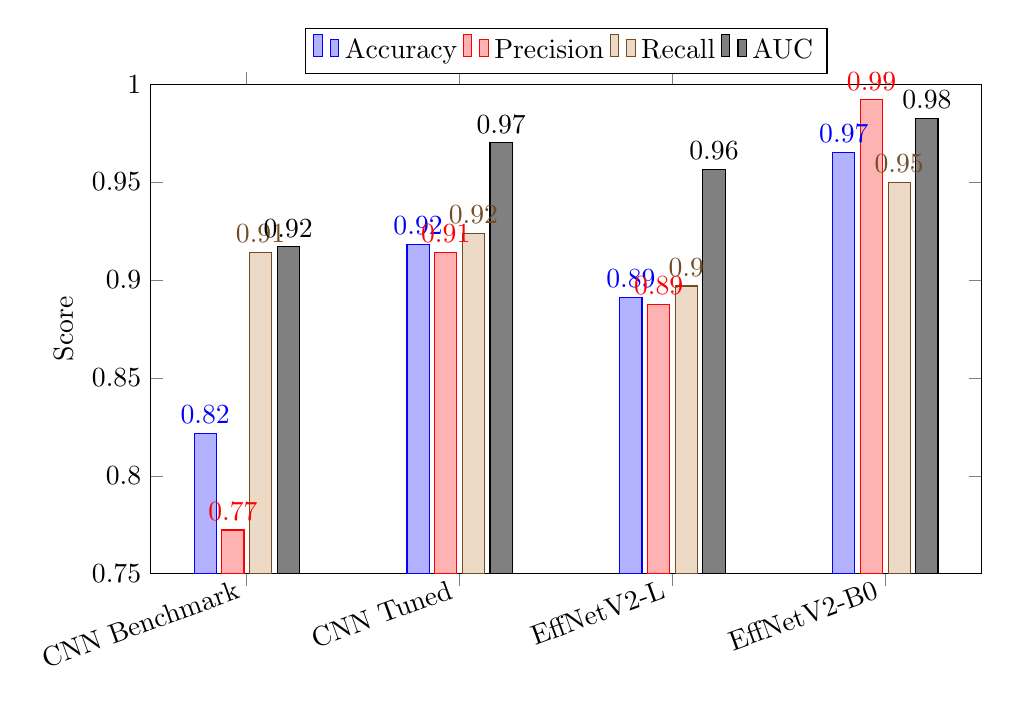
\begin{tikzpicture}
\begin{axis}[
    ybar,
    width=\textwidth,
    height=7.8cm,
    ymin=0.75,
    ymax=1.00,
    bar width=8pt,
    symbolic x coords={CNN Benchmark,CNN Tuned,EffNetV2-L,EffNetV2-B0},
    xtick=data,
    xticklabel style={rotate=20,anchor=east},
    ylabel={Score},
    legend style={at={(0.5,1.02)}, anchor=south, legend columns=-1},
    enlarge x limits=0.15,
    nodes near coords,
    nodes near coords align={vertical}
]
\addplot coordinates {(CNN Benchmark,0.8216) (CNN Tuned,0.9181) (EffNetV2-L,0.8912) (EffNetV2-B0,0.9651)};
\addplot coordinates {(CNN Benchmark,0.7723) (CNN Tuned,0.9142) (EffNetV2-L,0.8875) (EffNetV2-B0,0.9919)};
\addplot coordinates {(CNN Benchmark,0.9139) (CNN Tuned,0.9236) (EffNetV2-L,0.8969) (EffNetV2-B0,0.9498)};
\addplot coordinates {(CNN Benchmark,0.9169) (CNN Tuned,0.9700) (EffNetV2-L,0.9564) (EffNetV2-B0,0.9824)};
\legend{Accuracy,Precision,Recall,AUC}
\end{axis}
\end{tikzpicture}
\caption{EfficientNetV2-B0 emerged as the strongest preserved tradeoff in the experiment log.}
\label{fig:model-comparison}
\end{figure}

\subsubsection{Why EfficientNetV2-B0 was selected}
EfficientNetV2-B0 won for a practical reason: it delivered the strongest preserved validation performance without requiring the largest backbone. In a project constrained by dataset size, training time, and deployment complexity, that balance mattered.

The preserved notebook shows that the best model used:
\begin{itemize}[leftmargin=1.5em]
    \item \textbf{ImageNet weights},
    \item \textbf{include\_top=False},
    \item \textbf{pooling='max'},
    \item a final \textbf{Dense(1, activation='sigmoid')} output,
    \item \textbf{Adam} with a learning rate of \(\mathbf{1 \times 10^{-5}}\),
    \item and end-to-end fine-tuning with the backbone set to trainable.
\end{itemize}

That meant I was not using EfficientNet as a frozen feature extractor only. I was using transfer learning and then specializing the model to the deepfake task.

\subsubsection{Deployment architecture}
The deployed app is a Streamlit frontend. The repo includes:
\begin{itemize}[leftmargin=1.5em]
    \item an app entrypoint in \texttt{streamlit\_app.py},
    \item the main interface and inference logic in \texttt{app.py},
    \item a zipped pretrained model archive in \texttt{code/PretrainedModel/dffnetv2B0.zip},
    \item requirements and deployment instructions for Streamlit Community Cloud.
\end{itemize}

At startup, the app can extract the saved model, load the JSON architecture and H5 weights, preprocess the user image, and run local/server-side inference through TensorFlow/Keras.

\subsection{Work Product}

\subsubsection{What the work product actually is}
The work product is not only a notebook. It is the combination of:
\begin{enumerate}[leftmargin=1.5em]
    \item a trained and preserved image-level detector,
    \item a deployed web interface for image upload and inference,
    \item a technical analysis of how the model behaves,
    \item a documented conceptual pivot toward a broader authenticity system.
\end{enumerate}

That combination matters because the mini-capstone was supposed to be a \emph{real piece of work}, not only a concept sketch.

\subsubsection{Current system pipeline}
\begin{figure}[H]
\centering
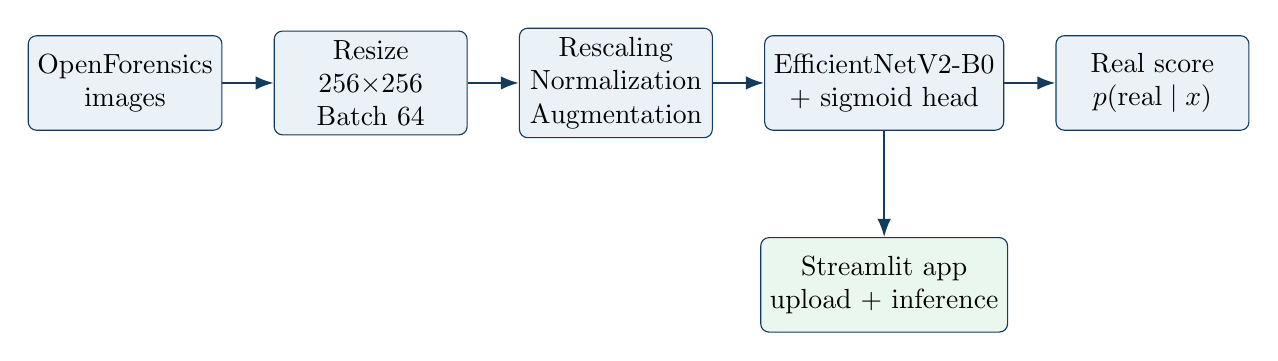
\begin{tikzpicture}[
    node distance=1.35cm and 0.65cm,
    box/.style={draw=navy, rounded corners=3pt, minimum width=2.45cm, minimum height=1.2cm, align=center, fill=softblue},
    arrow/.style={-{Latex[length=2.3mm]}, thick, draw=navy}
]
\node[box] (data) {OpenForensics\\images};
\node[box, right=of data] (prep) {Resize\\256$\times$256\\Batch 64};
\node[box, right=of prep] (aug) {Rescaling\\Normalization\\Augmentation};
\node[box, right=of aug] (model) {EfficientNetV2-B0\\+ sigmoid head};
\node[box, right=of model] (score) {Real score\\$p(\text{real}\mid x)$};
\node[box, below=of model, fill=softgreen] (deploy) {Streamlit app\\upload + inference};
\draw[arrow] (data) -- (prep);
\draw[arrow] (prep) -- (aug);
\draw[arrow] (aug) -- (model);
\draw[arrow] (model) -- (score);
\draw[arrow] (model) -- (deploy);
\end{tikzpicture}
\caption{First-iteration work product, from dataset pipeline to deployed detector.}
\label{fig:current-pipeline}
\end{figure}

\subsubsection{How the model works}
The first-iteration model is a binary image classifier that estimates:
\[
p = p(\text{real}\mid x)
\]
for an input image \(x\). The app then applies a threshold:
\[
p \ge 0.50 \Rightarrow \text{Real}, \qquad p < 0.50 \Rightarrow \text{Fake}
\]

The saved architecture shows:
\begin{enumerate}[leftmargin=1.5em]
    \item an input layer for \textbf{256 $\times$ 256 $\times$ 3} images,
    \item a \textbf{Rescaling} layer,
    \item a \textbf{Normalization} layer,
    \item an \textbf{EfficientNetV2-B0} backbone,
    \item a \textbf{GlobalMaxPooling2D} layer,
    \item a final \textbf{Dense} layer with one \textbf{sigmoid} unit.
\end{enumerate}

The network learns by minimizing binary cross-entropy:
\[
\mathcal{L}(y,p) = -\left[y\log(p) + (1-y)\log(1-p)\right]
\]
where \(y\) is the true label and \(p\) is the predicted real-image probability. In practice:
\begin{itemize}[leftmargin=1.5em]
    \item wrong predictions produce large loss,
    \item correct predictions reduce loss,
    \item backpropagation and Adam update the network weights,
    \item the filters gradually specialize toward the cues that separate the two classes.
\end{itemize}

What the model learns is a forensic notion of realism:
\begin{itemize}[leftmargin=1.5em]
    \item local texture irregularities,
    \item blending seams,
    \item abnormal high-frequency detail,
    \item inconsistent skin or hair statistics,
    \item generator-like artifacts.
\end{itemize}

That is powerful, but it is not the same thing as truth or authenticity.

\begin{figure}[H]
\centering
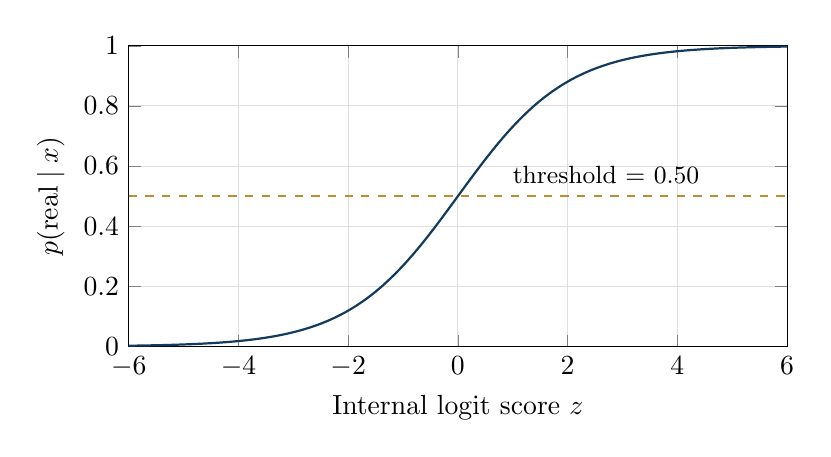
\begin{tikzpicture}
\begin{axis}[
    width=0.82\textwidth,
    height=5.4cm,
    xmin=-6,
    xmax=6,
    ymin=0,
    ymax=1,
    xlabel={Internal logit score $z$},
    ylabel={$p(\text{real}\mid x)$},
    samples=200,
    domain=-6:6,
    grid=major,
    grid style={gray!25}
]
\addplot[navy, thick] {1/(1+exp(-x))};
\addplot[dashed, gold, thick] coordinates {(-6,0.5) (6,0.5)};
\node at (axis cs:2.7,0.57) {\small threshold = 0.50};
\end{axis}
\end{tikzpicture}
\caption{Sigmoid output of the binary classifier. The app converts this probability into a Real/Fake label using the current 0.50 threshold.}
\label{fig:sigmoid-threshold}
\end{figure}

\subsection{Results / What I Got}

\subsubsection{Training behavior}
The preserved history for the best model shows that by the final recorded epoch it reached:
\begin{itemize}[leftmargin=1.5em]
    \item training loss: \textbf{0.0052},
    \item training accuracy: \textbf{0.9985},
    \item validation loss: \textbf{0.1196},
    \item validation accuracy: \textbf{0.9651}.
\end{itemize}

\begin{figure}[H]
\centering

\includegraphics[width=0.82\textwidth]{v2b0_history.png}
\caption{Saved training history for EfficientNetV2-B0.}
\label{fig:v2b0-history}
\end{figure}

\subsubsection{Validation and test results}
The preserved testing notebook reports:
\begin{itemize}[leftmargin=1.5em]
    \item test loss: \textbf{0.5126},
    \item test accuracy: \textbf{0.8577},
    \item test AUC: \textbf{0.9387},
    \item test precision: \textbf{0.9188},
    \item test recall: \textbf{0.7828}.
\end{itemize}

\begin{figure}[H]
\centering
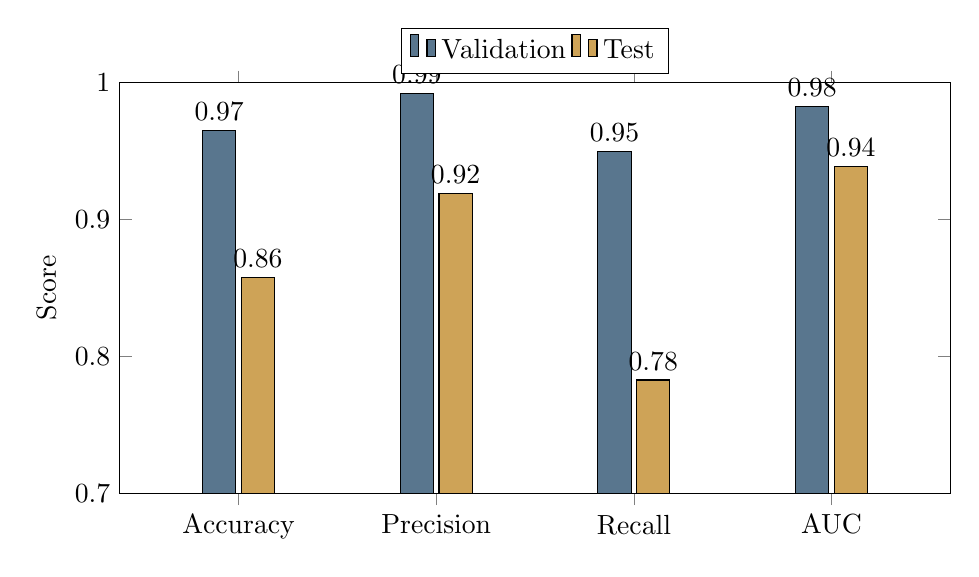
\begin{tikzpicture}
\begin{axis}[
    ybar,
    width=\textwidth,
    height=6.8cm,
    ymin=0.70,
    ymax=1.00,
    bar width=12pt,
    symbolic x coords={Accuracy,Precision,Recall,AUC},
    xtick=data,
    ylabel={Score},
    enlarge x limits=0.2,
    legend style={at={(0.5,1.02)}, anchor=south, legend columns=-1},
    nodes near coords,
    nodes near coords align={vertical}
]
\addplot[fill=navy!70] coordinates {(Accuracy,0.9651) (Precision,0.9919) (Recall,0.9498) (AUC,0.9824)};
\addplot[fill=gold!80] coordinates {(Accuracy,0.8577) (Precision,0.9188) (Recall,0.7828) (AUC,0.9387)};
\legend{Validation,Test}
\end{axis}
\end{tikzpicture}
\caption{Validation versus held-out test performance. This gap is one of the most important technical findings in the project.}
\label{fig:val-test-gap}
\end{figure}

\begin{figure}[H]
\centering
\begin{subfigure}[t]{0.48\textwidth}
    \centering
    
\includegraphics[width=\textwidth]{loss_acc.png}
    \caption{Loss and accuracy snapshot}
\end{subfigure}
\hfill
\begin{subfigure}[t]{0.48\textwidth}
    \centering
    
\includegraphics[width=\textwidth]{loss_precision.png}
    \caption{Loss and precision snapshot}
\end{subfigure}
\caption{Preserved evaluation plots from the original project artifacts.}
\label{fig:loss-panels}
\end{figure}

\begin{figure}[H]
\centering
\begin{subfigure}[t]{0.48\textwidth}
    \centering
    
\includegraphics[width=\textwidth]{precision_recall.png}
    \caption{Precision-recall curve}
\end{subfigure}
\hfill
\begin{subfigure}[t]{0.48\textwidth}
    \centering
    
\includegraphics[width=\textwidth]{v2b0_roc.png}
    \caption{ROC curve}
\end{subfigure}
\caption{Preserved precision-recall and ROC behavior for the selected model.}
\label{fig:eval-curves}
\end{figure}

\subsubsection{What worked}
Three things worked clearly:
\begin{enumerate}[leftmargin=1.5em]
    \item the detector achieved strong preserved validation metrics,
    \item the model-selection process identified a clear winner,
    \item the pipeline was strong enough to survive deployment into a user-facing app.
\end{enumerate}

\subsubsection{What did not work fully}
The most important limitation was that the model generalized less strongly to the harder test set than to the validation split. That gap suggests sensitivity to distribution shift, stronger perturbations, and post-processing artifacts. The repository notes that the harder data includes distortions such as noise, blur, and altered pixels. That means the model was robust, but not robust enough for authenticity on its own.

\subsubsection{The Gandhi failure case}
The most important qualitative result came after deployment. I tested the app with a visually plausible but historically impossible synthetic image: \textbf{Mahatma Gandhi taking a selfie}. The detector still leaned toward ``real.''

\callout{Why that case matters}{
The Gandhi selfie did not show that the detector was random. It showed that the detector was answering a narrower question than authenticity. It was reading visual plausibility, not historical possibility, claim consistency, or source trust.
}

\begin{figure}[H]
\centering
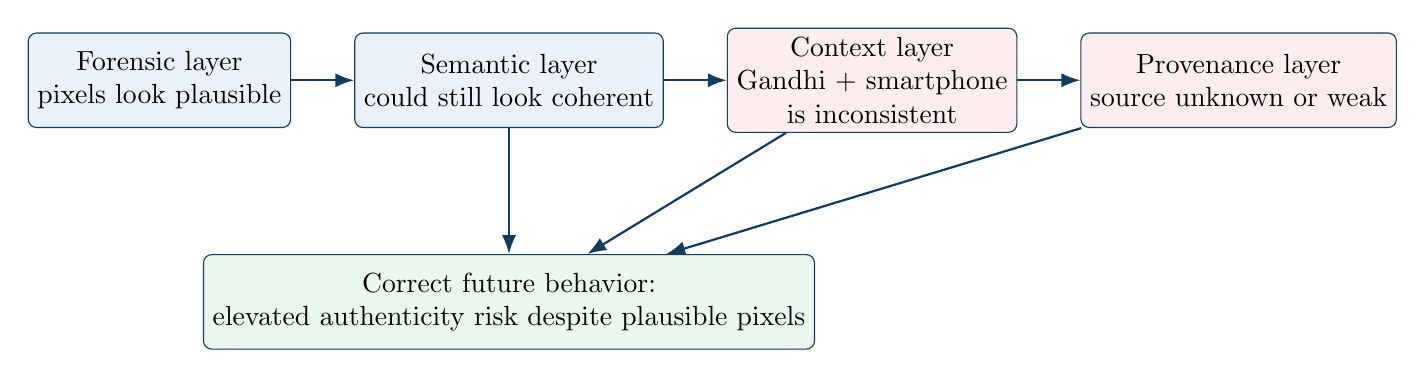
\begin{tikzpicture}[
    node distance=1.6cm and 0.8cm,
    box/.style={draw=navy, rounded corners=3pt, minimum width=2.85cm, minimum height=1.2cm, align=center, fill=softblue},
    bad/.style={draw=navy, rounded corners=3pt, minimum width=2.85cm, minimum height=1.2cm, align=center, fill=softred},
    good/.style={draw=navy, rounded corners=3pt, minimum width=2.85cm, minimum height=1.2cm, align=center, fill=softgreen},
    arrow/.style={-{Latex[length=2.4mm]}, thick, draw=navy}
]
\node[box] (a) {Forensic layer\\pixels look plausible};
\node[box, right=of a] (b) {Semantic layer\\could still look coherent};
\node[bad, right=of b] (c) {Context layer\\Gandhi + smartphone\\is inconsistent};
\node[bad, right=of c] (d) {Provenance layer\\source unknown or weak};
\node[good, below=of b, minimum width=4.6cm] (e) {Correct future behavior:\\elevated authenticity risk despite plausible pixels};
\draw[arrow] (a) -- (b);
\draw[arrow] (b) -- (c);
\draw[arrow] (c) -- (d);
\draw[arrow] (b) -- (e);
\draw[arrow] (c) -- (e);
\draw[arrow] (d) -- (e);
\end{tikzpicture}
\caption{Why the Gandhi selfie changed the project. A single forensic score is not enough; the contradiction appears when multiple evidence layers are considered together.}
\label{fig:gandhi-logic}
\end{figure}

\subsubsection{What I learned from the results}
The results led me to three conclusions:
\begin{enumerate}[leftmargin=1.5em]
    \item benchmark performance and authenticity are not the same thing,
    \item image forensics is necessary but not sufficient,
    \item failure cases are design instructions, not side notes.
\end{enumerate}

\subsection{General Plan Going Forward}

\subsubsection{The four-layer authenticity system}
The next iteration is an image-only authenticity analyzer with four evidence modules and a fusion layer.

\begin{figure}[H]
\centering
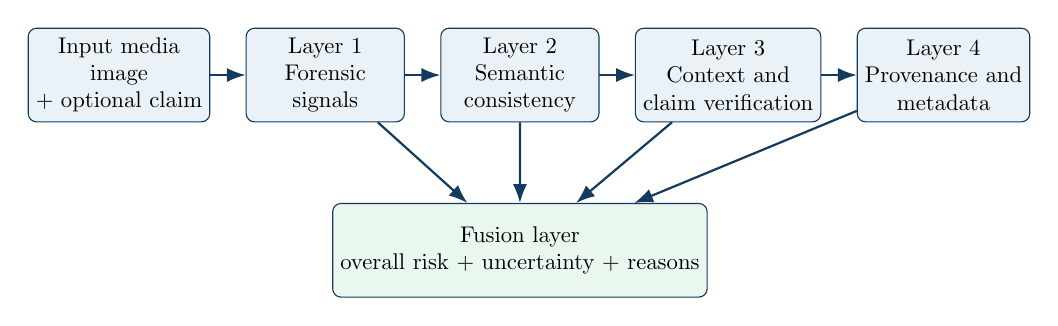
\begin{tikzpicture}[
    scale=0.82,
    transform shape,
    node distance=1.25cm and 0.55cm,
    box/.style={draw=navy, rounded corners=3pt, minimum width=2.45cm, minimum height=1.45cm, align=center, fill=softblue},
    arrow/.style={-{Latex[length=2.4mm]}, thick, draw=navy}
]
\node[box] (input) {Input media\\image\\+ optional claim};
\node[box, right=of input] (forensic) {Layer 1\\Forensic\\signals};
\node[box, right=of forensic] (semantic) {Layer 2\\Semantic\\consistency};
\node[box, right=of semantic] (context) {Layer 3\\Context and\\claim verification};
\node[box, right=of context] (prov) {Layer 4\\Provenance and\\metadata};
\node[box, below=of semantic, minimum width=4.8cm, fill=softgreen] (fusion) {Fusion layer\\overall risk + uncertainty + reasons};
\draw[arrow] (input) -- (forensic);
\draw[arrow] (forensic) -- (semantic);
\draw[arrow] (semantic) -- (context);
\draw[arrow] (context) -- (prov);
\draw[arrow] (forensic) -- (fusion);
\draw[arrow] (semantic) -- (fusion);
\draw[arrow] (context) -- (fusion);
\draw[arrow] (prov) -- (fusion);
\end{tikzpicture}
\caption{The proposed four-layer image authenticity system.}
\label{fig:shield-architecture}
\end{figure}

\paragraph{Layer 1: Forensic.}
The current EfficientNetV2-B0 detector already belongs here. In the next iteration, I want to add a \textbf{variational autoencoder (VAE)} \cite{kingma2014vae}. The VAE would add anomaly evidence by measuring reconstruction error and latent irregularity, not only classification confidence.

\paragraph{Layer 2: Semantic consistency.}
This layer asks whether the image makes internal sense. I want to use an attention-based or region-based approach \cite{vaswani2017attention} so the system can focus on hands, fingers, reflections, facial boundaries, and interaction regions rather than treating every patch equally.

\paragraph{Layer 3: Context and claim verification.}
This layer asks whether the image fits the claim being made about it. I want a narrow \textbf{retrieval-augmented generation (RAG)} style verifier \cite{lewis2020rag}. The purpose is not to let a language model guess history, but to retrieve facts and compare them against the image/claim pair.

\paragraph{Layer 4: Provenance and metadata.}
This layer asks whether there is trustworthy evidence about origin, editing history, or credentials. I am especially interested in metadata checks and future support for \textbf{C2PA Content Credentials} \cite{c2pa}.

\subsubsection{Dataset stack instead of one giant dataset}
This project now needs a \textbf{dataset stack}, because each layer answers a different question. The stack I want to use is:
\begin{itemize}[leftmargin=1.5em]
    \item \textbf{RAISE} for camera-native images \cite{raise},
    \item \textbf{OpenForensics} for face-forensics and manipulated imagery \cite{le2021openforensics},
    \item \textbf{Columbia Uncompressed} for clean splicing examples \cite{columbia},
    \item \textbf{GenImage} for AI-generated still images \cite{genimage},
    \item \textbf{NewsCLIPpings} plus a small \textbf{VisualNews} subset for context mismatch \cite{newsclippings,visualnews},
    \item a \textbf{custom paired subset} with original, non-AI edited, and AI-edited versions of the same source image.
\end{itemize}

\begin{figure}[H]
\centering
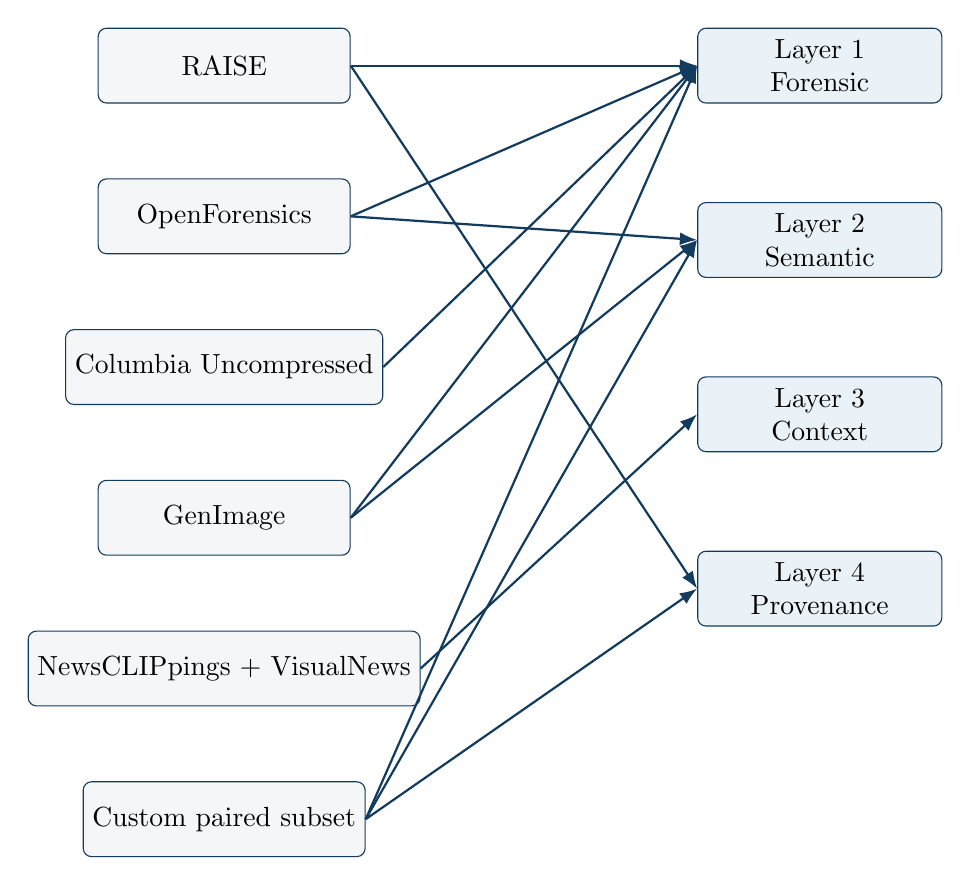
\begin{tikzpicture}[
    node distance=0.95cm and 1.0cm,
    ds/.style={draw=navy, rounded corners=3pt, minimum width=3.2cm, minimum height=0.95cm, align=center, fill=softgray},
    layer/.style={draw=navy, rounded corners=3pt, minimum width=3.1cm, minimum height=0.95cm, align=center, fill=softblue},
    arrow/.style={-{Latex[length=2.2mm]}, thick, draw=navy}
]
\node[ds] (raise) {RAISE};
\node[ds, below=of raise] (openf) {OpenForensics};
\node[ds, below=of openf] (columbia) {Columbia Uncompressed};
\node[ds, below=of columbia] (genimage) {GenImage};
\node[ds, below=of genimage] (news) {NewsCLIPpings + VisualNews};
\node[ds, below=of news] (custom) {Custom paired subset};

\node[layer, right=4.4cm of raise] (l1) {Layer 1\\Forensic};
\node[layer, below=1.25cm of l1] (l2) {Layer 2\\Semantic};
\node[layer, below=1.25cm of l2] (l3) {Layer 3\\Context};
\node[layer, below=1.25cm of l3] (l4) {Layer 4\\Provenance};

\draw[arrow] (raise.east) -- (l4.west);
\draw[arrow] (raise.east) -- (l1.west);
\draw[arrow] (openf.east) -- (l1.west);
\draw[arrow] (openf.east) -- (l2.west);
\draw[arrow] (columbia.east) -- (l1.west);
\draw[arrow] (genimage.east) -- (l1.west);
\draw[arrow] (genimage.east) -- (l2.west);
\draw[arrow] (news.east) -- (l3.west);
\draw[arrow] (custom.east) -- (l1.west);
\draw[arrow] (custom.east) -- (l2.west);
\draw[arrow] (custom.east) -- (l4.west);
\end{tikzpicture}
\caption{Dataset stack plan. Different datasets support different evidence layers; there is no single public dataset that cleanly covers the whole authenticity problem.}
\label{fig:dataset-stack}
\end{figure}

\subsubsection{Label taxonomy}
The output space should be more informative than only real versus fake.

\begin{table}[H]
\centering
\caption{Label taxonomy for the next iteration}
\label{tab:label-taxonomy}
\begin{tabular}{p{3.2cm}p{5.5cm}p{5.2cm}}
\toprule
Label & Definition & Relevant layer(s) \\
\midrule
\texttt{camera\_native} & Image captured directly from a camera pipeline with no known content-changing edits. & Forensic, Provenance \\
\texttt{non\_ai\_edited} & Image edited or composited without generative AI. & Forensic, Provenance \\
\texttt{ai\_generated} & Image generated from scratch by a generative model. & Forensic, Semantic \\
\texttt{ai\_edited} & Real image that has been modified with a generative tool. & Forensic, Semantic, Provenance \\
\texttt{context\_consistent} & Image and claim do not present an obvious contradiction. & Context \\
\texttt{context\_inconsistent} & Image and claim contradict each other or retrieved evidence. & Context \\
\texttt{not\_applicable} & No claim is present, so context verification is not applied. & Context \\
\texttt{provenance\_strong} & Source history or metadata strongly supports authenticity. & Provenance \\
\texttt{provenance\_weak} & Some origin information is present but incomplete. & Provenance \\
\texttt{provenance\_missing} & Important source information is absent. & Provenance \\
\texttt{provenance\_unknown} & The file cannot be confidently categorized from available evidence. & Provenance \\
\bottomrule
\end{tabular}
\end{table}

\subsubsection{Practical V1 roadmap}
I do not need to build the full future system at equal depth immediately. The practical next version is a \textbf{4-layer image-only V1}:
\begin{enumerate}[leftmargin=1.5em]
    \item keep the current EfficientNet detector as Layer 1,
    \item add a simple metadata/provenance checker,
    \item add a narrow semantic checker with regions or landmarks,
    \item add a narrow context verifier for claim-based contradictions,
    \item fuse all four signals into a final risk score.
\end{enumerate}

\begin{table}[H]
\centering
\caption{Current status versus next-step roadmap}
\label{tab:status-roadmap}
\begin{tabular}{p{4.8cm}p{2.1cm}p{7.0cm}}
\toprule
Component & Status & Meaning \\
\midrule
OpenForensics image pipeline & Completed & Stable loading, resizing, labeling, and preprocessing pipeline. \\
Model comparison across CNN families & Completed & Compared benchmark CNNs and transfer-learning candidates. \\
EfficientNetV2-B0 selection & Completed & Best preserved validation tradeoff in the repository. \\
Streamlit deployment & Completed & App for upload and inference. \\
Qualitative stress testing & Completed & Gandhi selfie exposed a scope limitation. \\
Provenance checker & Planned & Metadata and source-trust signals. \\
Semantic checker & Planned & Region consistency, hands, reflections, boundaries. \\
Context verifier & Planned & Claim-based contradiction checking. \\
Fusion layer & Planned & Final calibrated authenticity risk. \\
\bottomrule
\end{tabular}
\end{table}

\section{Part 3: Capstone Process Documentation}

\subsection{Overview}
This process section explains \emph{how} the project evolved, not only \emph{what} I built. The part I am proudest of is not only the final validation metric; it is that I used the deployed detector as a tool for discovering the real scope of the problem. The mini-capstone began as a deepfake detector and became a more mature authenticity project because I stress-tested it and let the failure case change my design.

\subsection{Modeling Professional Process}
One thing I learned from this project is that a professional machine learning workflow is rarely ``pick a fancy model and stop when the benchmark looks good.'' A more realistic process looks like this:
\begin{enumerate}[leftmargin=1.5em]
    \item define a narrow task,
    \item build or audit a usable pipeline,
    \item compare candidate models,
    \item deploy the strongest viable version,
    \item test it under harder real-world conditions,
    \item analyze failures,
    \item redesign the system around those failures.
\end{enumerate}

That sequence fits this project closely. I started with a narrow image-level problem because it was buildable, measurable, and compatible with the preserved repository artifacts. Only after the detector existed and could be stress-tested did it become clear what a broader authenticity system should contain.

This is also why I kept the current work product focused. A capstone has to be ambitious, but it also has to be finishable. The detector was the completed product. The four-layer authenticity shield is the next design built out of the detector's limitations.

\subsection{Additional Learning Not Directly Visible in the Work Product}
The deployed detector is only part of what I learned. A large amount of additional learning happened in support of the work product and shaped the future design:
\begin{itemize}[leftmargin=1.5em]
    \item I read method papers on transfer learning, VAEs, attention, and RAG so I could decide what kinds of models belong in later layers.
    \item I studied dataset documentation to understand that authenticity cannot be trained from a single public corpus and instead requires a dataset stack.
    \item I learned more about provenance and content credentials than the current app visibly uses, because that is necessary for the next iteration even if the first detector does not implement it yet.
    \item I learned more about deployment environments than is obvious from the model notebook alone, especially dependency pinning, Python version constraints, and TensorFlow packaging.
\end{itemize}

That learning is important because it explains why the future system design is not arbitrary. It is grounded in research and implementation constraints that I had to study even when the current work product could not yet incorporate all of them.

\subsection{Use of Generative AI}
Generative AI was part of my process, but not a substitute for actual engineering work. I used it in four main ways:
\begin{enumerate}[leftmargin=1.5em]
    \item to brainstorm architecture options after the Gandhi failure case,
    \item to pressure-test how to explain advanced methods such as VAEs, attention, and RAG accessibly,
    \item to reason through deployment issues and likely compatibility failures,
    \item to help structure and rewrite documentation for different audiences.
\end{enumerate}

I also used AI indirectly through the project itself: AI-generated images became part of the problem, the test cases, and the conceptual argument of the capstone.

\paragraph{Where AI helped.}
AI was especially useful for:
\begin{itemize}[leftmargin=1.5em]
    \item turning rough ideas into alternative architectures,
    \item surfacing likely deployment problems quickly,
    \item helping me compare whether a section was too technical or too vague,
    \item proposing ways to connect the first detector to a broader system.
\end{itemize}

\paragraph{Where AI could mislead.}
AI could also mislead badly if used uncritically. It can:
\begin{itemize}[leftmargin=1.5em]
    \item overclaim what one detector can do,
    \item compress different authenticity problems into one label,
    \item invent dataset coverage that is not really there,
    \item produce polished but unsupported methodological claims.
\end{itemize}

\paragraph{How I checked AI suggestions.}
I treated AI suggestions as hypotheses, not facts. I checked them against:
\begin{itemize}[leftmargin=1.5em]
    \item the actual repository notebooks and CSVs,
    \item the saved app code and deployment files,
    \item official dataset pages and method papers,
    \item the performance numbers preserved in the repo,
    \item what the deployed app actually did in practice.
\end{itemize}

\paragraph{How Gandhi/Sora-style examples shaped the project.}
The Gandhi selfie example did not come from a benchmark. It came from using generated media as an adversarial stress test. That is one of the places where generative AI changed the process directly: it became both the object of detection and the mechanism for exposing the detector's conceptual limits.

\subsection{Strategies for \#navigation}
The hardest navigation problem in this project was scope. I initially had a broad instinct to build some version of an ``AI shield,'' but that idea was too large to be a good mini-capstone starting point. The successful navigation move was to narrow first:
\begin{itemize}[leftmargin=1.5em]
    \item start with one buildable layer,
    \item complete it end to end,
    \item then use failure to decide what should come next.
\end{itemize}

\paragraph{How I handled setbacks.}
The major setbacks were:
\begin{itemize}[leftmargin=1.5em]
    \item the scale of the image data,
    \item the fact that the repository preserved artifacts but not every intermediate decision,
    \item deployment issues after the model itself was already selected,
    \item the conceptual discomfort of discovering that a strong detector still answered the wrong question for some cases.
\end{itemize}

I handled those setbacks by narrowing aggressively, preserving the strongest available evidence, and separating what was complete from what was planned.

\paragraph{What I would do differently next time.}
If I were starting again, I would define the multi-layer label space earlier. I would also build a curated challenge set in parallel with model training rather than after deployment. That would have surfaced the ``forensics vs authenticity'' distinction sooner.

\subsection{HC/LO Reflection}
The main takeaway from the HCs and LOs in this project is that the capstone became better not because I knew one advanced neural network, but because I kept moving between \textbf{modeling}, \textbf{evidence}, \textbf{engineering constraints}, and \textbf{audience-aware communication}. The project improved when I used those skills together.

The most important surprise for me was that some of the most useful habits were not the glamorous ones. \textbf{\#organization}, \textbf{\#professionalism}, and \textbf{\#navigation} mattered as much as the machine learning content. Without them, I would have had a benchmark summary and a half-working app, not a coherent capstone story.

\subsection{HC Descriptions}
I am grouping the HCs by how they functioned in the project rather than presenting them as a random list. This makes the process easier to follow.

\subsubsection*{Problem framing and modeling}
\paragraph{\#breakitdown}
This project only became tractable when I decomposed ``build an AI shield'' into smaller, separable questions. First I asked whether I could build a deployable image-level detector. Only after that did I separate forensic, semantic, contextual, and provenance evidence into distinct layers.

\paragraph{\#modeltypes}
This HC mattered when I realized that one classifier could not answer every authenticity question. It helped me distinguish between a supervised classifier, an anomaly model such as a VAE, an attention-based semantic checker, and a retrieval-backed context system as different model types serving different roles.

\paragraph{\#constraints}
Constraint-awareness shaped nearly every decision. Dataset size, training cost, deployment compatibility, and the realities of a mini-capstone all pushed me toward a narrower first iteration and a staged plan for the broader system.

\paragraph{\#abstraction}
I used abstraction when I shifted from one failing example to a system-level insight. Gandhi taking a selfie was not only one bad prediction; it was an abstract demonstration that visual realism and authenticity are different problem classes.

\subsubsection*{Analysis and decision-making}
\paragraph{\#estimation}
Estimation mattered when deciding what was feasible within the time and compute budget. It also mattered when reading results: a near-perfect validation score did not mean the model was universally trustworthy once I considered the likely scale of distribution shift.

\paragraph{\#induction}
I used induction when moving from repeated model behavior and preserved metrics to broader conclusions about what the detector had learned. I also used it carefully when deciding that the Gandhi test revealed a systematic limitation rather than an isolated glitch.

\paragraph{\#utility}
This HC mattered in trade-off decisions. I had to weigh whether it was better to chase a marginally stronger model, keep the smaller EfficientNetV2-B0, or invest time in deployment and evaluation. I chose the path that increased the usefulness of the project as a capstone.

\paragraph{\#evidence}
The project improved when I forced claims to stay tied to evidence. I checked architecture details against saved files, numerical claims against CSVs, deployment claims against the actual app code, and strategic claims against the model's observed failure modes.

\subsubsection*{Implementation and debugging}
\paragraph{\#iteration}
The whole project is iterative by structure. I did not treat the first detector as the final answer. I treated it as a first build, then revised the project after deployment and stress testing.

\paragraph{\#debugging}
Debugging appeared both in code and in concepts. On the code side, deployment required dependency and compatibility fixes. On the conceptual side, I had to debug my own framing of the problem after the Gandhi case exposed that ``deepfake detection'' was too narrow.

\paragraph{\#tradeoffs}
This HC appeared repeatedly in model choice, deployment choice, and writing choice. I consistently had to choose between breadth and depth, larger and smaller backbones, perfect scope and finished scope, ambitious language and accurate language.

\subsubsection*{Communication and organization}
\paragraph{\#organization}
Organization shaped the data pipeline, the experiment comparison, the app structure, and the report itself. The current document exists because I organized the work product, process material, and future plan into one readable structure instead of letting them remain scattered across notebooks, code, and ideas.

\paragraph{\#professionalism}
Professionalism mattered in being explicit about what was completed, what was planned, and what failed. It also meant treating deployment and documentation as part of the project rather than as optional presentation layers.

\paragraph{\#audience}
The assignment requires multiple audiences in one document, and this HC was central to that task. I had to explain the same project in general language for the Executive Summary, technical language for the academic sections, and reflective language for the Process Documentation.

\subsubsection*{Reflection and revision}
\paragraph{\#outcomefocus}
Even though this capstone is academic, I kept treating it as an outcomes-driven project. The detector had to exist, run, and produce interpretable behavior. The final story had to emerge from what the system actually did, not from what I hoped it would prove.

\paragraph{\#revision}
Revision was not cosmetic. I revised the conceptual scope of the project, the deployment design, and the way I explained the work after seeing where the first framing was too defensive or too superficial.

\paragraph{\#uncertainty}
This HC mattered because machine learning outputs are probabilistic and incomplete. Instead of pretending the model gave ground truth, I now see uncertainty as a first-class output of the future system.

\subsection{LO Descriptions}
The LO mapping below includes the four capstone LOs plus six Computational Sciences-aligned outcomes. For the Computational Sciences entries, I am mapping the project to the public descriptions of the relevant course areas because exact section-level LO wording can vary by course instance \cite{minervacs}.

\begin{longtable}{p{3.1cm}p{4.9cm}p{6.8cm}}
\caption{LO mapping for the mini-capstone}\label{tab:lo-mapping}\\
\toprule
LO & What the LO means in this project & Evidence from the capstone \\
\midrule
\endfirsthead
\toprule
LO & What the LO means in this project & Evidence from the capstone \\
\midrule
\endhead
\texttt{\#qualitydeliverables} & Produce a polished final deliverable with clear evidence of quality. & Deployed Streamlit app, polished single-document report, integrated figures, and a coherent project narrative. \\

\texttt{\#curation} & Select what belongs in the final submission and what should be omitted. & I narrowed the story to the strongest model, the most relevant plots, and the Gandhi failure case instead of trying to present every artifact equally. \\

\texttt{\#navigation} & Manage scope, setbacks, and evolving project conditions. & I began with a narrow detector, handled deployment setbacks, and used failure to redirect the project toward a layered authenticity system. \\

\texttt{\#outcomeanalysis} & Evaluate results honestly and draw defensible conclusions. & I interpreted the validation/test gap, documented what the Gandhi case meant, and separated completed work from planned future work. \\

\textbf{CS110-aligned: computational problem decomposition} & Break large technical problems into tractable components and choose workable representations. & I decomposed ``AI shield'' into detector, deployment, and then four future evidence layers rather than trying to build everything at once. \\

\textbf{CS114-aligned: probabilistic reasoning and uncertainty} & Interpret uncertainty, distributions, and model scores correctly. & I explained sigmoid outputs, thresholding, and why probabilistic scores should not be treated as absolute truth. \\

\textbf{CS130-aligned: predictive modeling and evaluation} & Build and assess predictive models using performance metrics and trade-offs. & I compared model candidates using validation metrics and interpreted the consequences of test degradation under harder data conditions. \\

\textbf{CS156-aligned: machine learning model construction and comparison} & Apply machine learning techniques and reason about generalization, overfitting, and performance. & The work product centers on a CNN classifier, transfer learning, preserved histories, and the interpretation of validation versus test behavior. \\

\textbf{CS162-aligned: software engineering and deployment} & Turn a computational model into a usable software artifact. & I moved the model into a Streamlit interface, handled dependency/version issues, and documented the deployment path for local and cloud use. \\

\textbf{CS166-aligned: complex systems modeling} & Understand systems in terms of interacting components rather than single variables. & The next iteration reframes authenticity as a system of interacting forensic, semantic, contextual, and provenance signals. \\
\bottomrule
\end{longtable}

\subsection{Timeline}
The timeline below shows the real sequence of the project rather than an idealized one.

\begin{figure}[H]
\centering
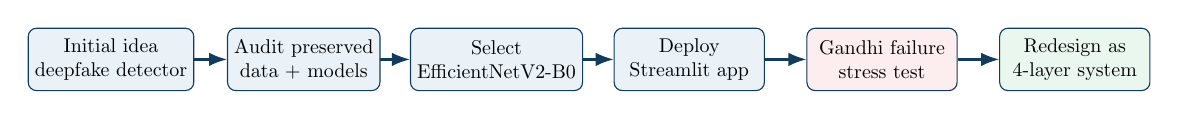
\begin{tikzpicture}[
    scale=0.72,
    transform shape,
    phase/.style={draw=navy, rounded corners=3pt, minimum width=2.65cm, minimum height=1.1cm, align=center, fill=softblue},
    arrow/.style={-{Latex[length=2.3mm]}, thick, draw=navy}
]
\node[phase] (a) at (0,0) {Initial idea\\deepfake detector};
\node[phase] (b) at (3.4,0) {Audit preserved\\data + models};
\node[phase] (c) at (6.8,0) {Select\\EfficientNetV2-B0};
\node[phase] (d) at (10.2,0) {Deploy\\Streamlit app};
\node[phase, fill=softred] (e) at (13.6,0) {Gandhi failure\\stress test};
\node[phase, fill=softgreen] (f) at (17.0,0) {Redesign as\\4-layer system};
\draw[arrow] (a) -- (b);
\draw[arrow] (b) -- (c);
\draw[arrow] (c) -- (d);
\draw[arrow] (d) -- (e);
\draw[arrow] (e) -- (f);
\end{tikzpicture}
\caption{Project timeline by phase. The redesign happened after deployment and stress testing, not before.}
\label{fig:timeline}
\end{figure}

\subsection{What challenges I faced and how I handled them}
The project faced four main challenges:
\begin{enumerate}[leftmargin=1.5em]
    \item \textbf{Data scale.} The full OpenForensics release is large, and even the preserved working split was big enough to make storage, file organization, and loading real constraints.
    \item \textbf{Training and compute.} The project had to balance batch size, model depth, and training practicality. That made EfficientNetV2-B0 attractive as a strong but not unnecessarily heavy backbone.
    \item \textbf{Deployment friction.} The deployment environment required its own engineering layer. TensorFlow package choices, Python versioning, and Streamlit compatibility all had to be handled explicitly. In the repo, this appears in the pinned requirements, the CPU TensorFlow build for non-Windows deployment, the Python 3.11 deployment guidance, and the app-entrypoint setup.
    \item \textbf{Scope correction.} The hardest challenge was accepting that a good first detector did not solve the full problem I cared about. I handled that by turning the failure into the center of the next design instead of hiding it.
\end{enumerate}

\subsection{How this project was different because of Minerva HCs and LOs}
Without the HCs and LOs, I could still have run a model and reported a score. What changed because of Minerva training was the quality of the analysis and the way I framed the outcome. Instead of treating the app as the end of the project, I treated it as one layer of a broader system and used structured reflection to explain why. That is the strongest sign, to me, that this work sits on top of the broader Minerva curriculum rather than only on top of one ML notebook.

\section{Conclusion}
This mini-capstone contains a complete first-iteration work product: a deployed deepfake image detector built around EfficientNetV2-B0, supported by preserved training artifacts, evaluation plots, and a technical explanation of how the model works.

It also contains the reason the project now needs to become something larger. The Gandhi selfie stress test showed that strong image-level forensics still leaves a gap between \emph{visual plausibility} and \emph{authenticity}. That gap is now the core intellectual contribution of the project.

So the final shape of the capstone is this:
\begin{enumerate}[leftmargin=1.5em]
    \item I built a complete first-layer detector.
    \item I used its limitations to define a more mature next iteration: a four-layer authenticity system built from forensic, semantic, contextual, and provenance evidence.
\end{enumerate}

That makes the project both concrete and forward-looking, which is exactly what I wanted from the mini-capstone.

\section{Appendix-Style Supporting Visuals}
The repository also preserves earlier presentation artifacts. I am including them here because they show the progression of the project, even though the current report is more complete.

\begin{figure}[H]
\centering
\begin{subfigure}[t]{0.32\textwidth}
    \centering
    
\includegraphics[width=\textwidth]{image2.jpg}
    \caption{Early problem/solution framing}
\end{subfigure}
\hfill
\begin{subfigure}[t]{0.32\textwidth}
    \centering
    
\includegraphics[width=\textwidth]{image1.jpg}
    \caption{Early model ranking summary}
\end{subfigure}
\hfill
\begin{subfigure}[t]{0.32\textwidth}
    \centering
    
\includegraphics[width=\textwidth]{image0.jpg}
    \caption{Early takeaways and future notes}
\end{subfigure}
\caption{Preserved presentation artifacts from the earlier iteration of the project.}
\label{fig:old-artifacts}
\end{figure}

\begin{thebibliography}{99}

\bibitem{le2021openforensics}
T.-N. Le, H. H. Nguyen, J. Yamagishi, and I. Echizen,
\emph{OpenForensics: Large-Scale Challenging Dataset for Multi-Face Forgery Detection and Segmentation In-The-Wild},
ICCV, 2021.
Dataset page: \url{https://zenodo.org/records/5528418}

\bibitem{tan2021efficientnetv2}
M. Tan and Q. V. Le,
\emph{EfficientNetV2: Smaller Models and Faster Training},
ICML, 2021.
\url{https://research.google/pubs/efficientnetv2-smaller-models-and-faster-training/}

\bibitem{kingma2014vae}
D. P. Kingma and M. Welling,
\emph{Auto-Encoding Variational Bayes},
ICLR, 2014.
\url{https://arxiv.org/abs/1312.6114}

\bibitem{vaswani2017attention}
A. Vaswani, N. Shazeer, N. Parmar, J. Uszkoreit, L. Jones, A. N. Gomez, {\L}. Kaiser, and I. Polosukhin,
\emph{Attention Is All You Need},
NeurIPS, 2017.
\url{https://arxiv.org/abs/1706.03762}

\bibitem{lewis2020rag}
P. Lewis, E. Perez, A. Piktus, F. Petroni, V. Karpukhin, N. Goyal, H. K\"uttler, M. Lewis, W.-t. Yih, T. Rockt\"aschel, S. Riedel, and D. Kiela,
\emph{Retrieval-Augmented Generation for Knowledge-Intensive NLP Tasks},
arXiv, 2020.
\url{https://arxiv.org/abs/2005.11401}

\bibitem{c2pa}
Coalition for Content Provenance and Authenticity (C2PA),
\emph{Content Credentials Technical Specification},
accessed April 2026.
\url{https://spec.c2pa.org/specifications/specifications/2.4/specs/C2PA_Specification.html}

\bibitem{raise}
D. Shullani, M. Fontani, T. Bianchi, A. De Rosa, A. Piva, and M. Barni,
\emph{RAISE: A Raw Images Dataset for Digital Image Forensics},
Proceedings of the ACM Multimedia Systems Conference, 2017.
Dataset page: \url{https://loki.disi.unitn.it/RAISE/}

\bibitem{columbia}
H. Farid,
\emph{Columbia Uncompressed Image Splicing Detection Evaluation Dataset},
Columbia University.
\url{https://www.ee.columbia.edu/ln/dvmm/downloads/authsplcuncmp/}

\bibitem{genimage}
Z. Zhu, Z. Wang, X. Wang, S. Zhao, and J. Lyu,
\emph{GenImage: A Million-Scale Benchmark for Detecting AI-Generated Images},
project page.
\url{https://genimage-dataset.github.io/}

\bibitem{visualnews}
F. Liu, A. Y. Lee, and Y. Lu,
\emph{VisualNews: Benchmark and Challenges in News Image Captioning},
project repository.
\url{https://github.com/FuxiaoLiu/VisualNews-Repository}

\bibitem{newsclippings}
A. L. B. Do, D. Roh, J. Lee, and A. G. Hauptmann,
\emph{NewsCLIPpings: Automatic Generation of Out-of-Context Multimodal Media},
EMNLP, 2021.
\url{https://aclanthology.org/2021.emnlp-main.545/}

\bibitem{hcintro}
Minerva University,
\emph{An Introduction to Habits of Mind and Foundational Concepts},
\url{https://www.minerva.edu/public/media/enrollment-center/Minerva-HCs-Intro.pdf}

\bibitem{minervacs}
Minerva University,
\emph{Computational Sciences Course Explorer},
\url{https://my.minerva.edu/academics/course_catalog/computational_sciences/}

\end{thebibliography}

\end{document}
